\documentclass{article}

\usepackage[preprint]{neurips_2024}
\usepackage[utf8]{inputenc}
\usepackage[T1]{fontenc}
\usepackage{hyperref}
\usepackage{url}
\usepackage{booktabs}
\usepackage{amsfonts}
\usepackage{nicefrac}
\usepackage{microtype}
\usepackage{xcolor}
\usepackage{graphicx}
\usepackage{algorithm}
\usepackage{algpseudocode}
\usepackage{amsmath}
\usepackage{float}


\title{Differential Privacy in Image Classification using ResNet-20 and DP-SGD, DP-Adam, and DP-RMSProp Optimization techniques}

\author{
    Praveen Rangavajhula\\
    Department of Computer Science\\
    University of Georgia\\
    Athens, GA, 30602\\
    \texttt{praveen.rangavajhula@uga.edu} \\
    \And
    Alexander Darwiche\\
    Department of Computer Science\\
    University of Georgia\\
    Athens, GA, 30605 \\
    \texttt{alexander.darwiche@uga.edu} \\
    \And
    Deven Allen\\
    Department of Computer Science\\
    University of Georgia\\
    Athens, GA, 30605 \\
    \texttt{dca09692@uga.edu} \\
}

\begin{document}

    \maketitle
    \begin{abstract}
    

    \end{abstract}


    \section{Introduction}\label{sec:introduction}
    
    Stochastic Gradient Descent (SGD) and its differentially private (DP) relative DP-SGD are frequently used optimizers for image classification tasks. DP-SGD
    introduces noise and gradient clipping to the standard SGD algorithm, to ensure that the underlying data remains private upon release of model parameters/hyperparameters. While DP-SGD
    is perhaps the most popular optimizer for tasks concerned with differential privacy, we also explore 2 additional optimization techniques. In this interim report, 
    we looked to explore the impact of changing the optimizer on the test accuracy achieveable on the CIFAR-10 dataset.
  
    The first additional optimizers tested in this paper are Differentially Private Root Mean Square Propogation (DP-RMSProp) and Adaptive Moment Estimation (DP-Adam). The motivation to try these optimizers is to properly bound
    the benefit of employing different optimization techniques from DP-SGD. RMSProp improves on SGD in that it includes a moving average of squared gradients. This additional term attempts to lessen the possibility of the
    vanishing/exploding gradient phenomenon. Adam, similarly, includes an estimation of first and second moment of gradients. Adam attempts to build on and improve on both RMSProp and AdaGrad \cite{kingma2017adammethodstochasticoptimization}.

    While implementing these additional optimizers is not novel unto itself, we believe it provides a solid groundwork for additional novelty and testing going forward. This interim report will
    highlight the current results of our testing and the anticipated path forward. We will briefly describe our proposed transition to a new optimization technique called Lion. To ensure Lion satisfies
    differential privacy, we will need to make adjustments, specifically by adding noise and clipping.

    \section{Formal Description of Models Tried}\label{sec:models}
    \subsection{Motivation and Rationale}\label{subsec:motivation-and-rationale}

As mentioned, the motivation for trying these optimizers was to appropriately bound the strength of the 3 optimization techniques for CIFAR-10. 
This lays a strong groundwork for future additions to the algorithms and allows us to have a wide range of options in making these adjustments. 

DP-SGD is likely the most common optimization algorithm used in differentially private image classification. The motivation for using DP-SGD is simply to have a strong 
baseline for comparison. Most literature regarding differential privacy begins by using DP-SGD, so it would make sense as the first algorithm implemented and tested.

RMSProp and Adam can be viewed as successors to DP-SGD. Both introduce approaches that allow for adaptivity of the step size taken at each iteration of the algorithm. These algorithms
were first proposed to deal with the vanishing/exlpoding gradient phenomenon and have now been used frequently in the differentially private image classification literature. We felt that
implementing these algorithms would provide us with a strong bound on the performance benefits associated with changing optimizer, essentially treating optimizers as another hyperparameter
that we could tune.

\subsection{Description of Optimization Algorithm (Psuedocode)}\label{subsec:algorithm-description}

Below are pseudocodes for the DP-SGD, DP-RMSprop, and DP-Adam algorithms that we plan to privatize, adapted or referenced from~\cite{DBLP:journals/corr/abs-1807-06766}:

\begin{algorithm}[H]
    \caption{DP-SGD}
    \label{alg:sgd}
    \begin{algorithmic}[1]
        \State \textbf{Input:} A step size $\alpha$, initial starting point $\mathbf{x}_1 \in \mathbb{R}^d$,
        and access to a (possibly noisy) oracle for gradients of $f : \mathbb{R}^d \rightarrow \mathbb{R}$.
        \State Initialize: $\mathbf{v}_0 = \mathbf{0}$
        \For{$t = 1, 2, \dots$}
            \State Compute gradient $\mathbf{g}_t = \nabla f(\mathbf{x}_t)$
            \State Clip gradient $\mathbf{g}_t = \mathbf{g}_t / \max(1, \frac{\lVert \mathbf{g}_t \rVert_2}{C})$
            \State Add noise: $\hat{\mathbf{g}}_t = \mathbf{g}_t + \mathcal{N}(0, \sigma^2 C^2 I)$
            \State Descent: $\mathbf{x}_{t+1} = \mathbf{x}_t - \alpha \hat{\mathbf{g}}_t$
        \EndFor
    \end{algorithmic}
\end{algorithm}

\begin{algorithm}[H]
    \caption{DP-RMSProp}
    \label{alg:rmsprop}
    \begin{algorithmic}[1]
        \State \textbf{Input:} A constant vector $\mathbb{R}^d \ni \xi \mathbf{1}_d \geq 0$, parameter $\beta_2 \in [0, 1)$, step size $\alpha$, initial starting point $\mathbf{x}_1 \in \mathbb{R}^d$, and access to a (possibly noisy) oracle for gradients of $f : \mathbb{R}^d \rightarrow \mathbb{R}$.
        \State Initialize: $\mathbf{v}_0 = \mathbf{0}$
        \For{$t = 1, 2, \dots$}
            \State Compute gradient $\mathbf{g}_t = \nabla f(\mathbf{x}_t)$
            \State Clip gradient $\mathbf{g}_t = \mathbf{g}_t / \max(1, \frac{\lVert \mathbf{g}_t \rVert_2}{C})$
            \State Add noise: $\hat{\mathbf{g}}_t = \mathbf{g}_t + \mathcal{N}(0, \sigma^2 C^2 I)$
            \State Calculate moving average of squared gradient $\mathbf{v}_t = \beta_2 \mathbf{v}_{t-1} + (1 - \beta_2)(\hat{\mathbf{g}}_t^2 + \xi \mathbf{1}_d)$
            \State Descent: $\mathbf{x}_{t+1} = \mathbf{x}_t - \alpha \mathbf{V}_t^{-1/2} \hat{\mathbf{g}}_t$
        \EndFor
    \end{algorithmic}
\end{algorithm}

\begin{algorithm}[H]
    \caption{DP-Adam}
    \label{alg:adam}
    \begin{algorithmic}[1]
        \State \textbf{Input:} A constant vector $\mathbb{R}^d \ni \xi \mathbf{1}_d > 0$, parameters $\beta_1, \beta_2 \in [0, 1)$, a sequence of step sizes $\{\alpha_t\}_{t=1,2,\dots}$, initial starting point $\mathbf{x}_1 \in \mathbb{R}^d$, and oracle access to gradients of $f : \mathbb{R}^d \rightarrow \mathbb{R}$.
        \State Initialize: $\mathbf{m}_0 = \mathbf{0}$, $\mathbf{v}_0 = \mathbf{0}$
        \For{$t = 1, 2, \dots$}
            \State Compute gradient $\mathbf{g}_t = \nabla f(\mathbf{x}_t)$
            \State Clip gradient: $\mathbf{g}_t = \mathbf{g}_t / \max(1, \frac{\lVert \mathbf{g}_t \rVert_2}{C})$
            \State Add noise: $\hat{\mathbf{g}}_t = \mathbf{g}_t + \mathcal{N}(0, \sigma^2 C^2 I)$
            \State Calculate moving average of squared gradient: $\mathbf{v}_t = \beta_2 \mathbf{v}_{t-1} + (1 - \beta_2)(\hat{\mathbf{g}}_t^2 + \xi \mathbf{1}_d)$
            \State Calculate moving average of gradient: $\mathbf{m}_t = \beta_1 \mathbf{m}_{t-1} + (1 - \beta_1) \hat{\mathbf{g}}_t$
            \State Descent: $\mathbf{x}_{t+1} = \mathbf{x}_t - \alpha_t \frac{\mathbf{m}_t}{\sqrt{\mathbf{v}_t} + \epsilon}$
        \EndFor
    \end{algorithmic}
\end{algorithm}


\subsection{Proposed Modifications and Variations}\label{subsec:modification-and-variations}
Most of our current work has focused on implementing and testing the existing DP-SGD, DP-RMSProp, and DP-Adam optimization techniques. The main axes
of testing involved changing hyperparameters like epsilon, batch size, or noise level. This has allowed us to establish a base with 3 optimization techniques
that can each be used to test our proposed modifications and variations going forward.

Our next proposed approach will be privatizing Evolved Sign Momentum (Lion) optimizer. This optimization technique builds on variants of SGD and Adam and having 
differentially private implementations, of those, available should provide a good basis of comparison for our newly privatized version of Lion, DP-Lion. In the private world,
DP-SGD is still the most popular optimization technique, however in the non-private world, versions of Adam (AdamW) or Adafactor are the usual choices for training
a deep neural netwrok. \cite{chen2023symbolicdiscoveryoptimizationalgorithms} We feel that transitioning from the primary private optimizer to a newly privatized Lion optimizer
will be an interesting approach to examine.

To privatize Lion, we will need to add gaussian noise that is relative to the number of iterations, epsilon, and sensitivity. This will take a very similar form to the privatization
done for DP-SGD, DP-RMSProp, and DP-Adam. Next, we also plan to implement a clipping constant C, so as to properly bound the sensitivity associated with neighboring datasets. The following psuedocode
introduces our proposed adjustments to the Lion Optimizer from~\cite{chen2023symbolicdiscoveryoptimizationalgorithms}.


\begin{algorithm}
    \caption{DP-Lion}
    \label{alg:lion}
    \begin{algorithmic}[1]
        \State \textbf{Input:} A constant vector $\mathbb{R}^d \ni \xi \mathbf{1}_d > 0$, parameters $\beta_1, \beta_2 \in [0, 1)$, a sequence of step sizes $\{\alpha_t\}_{t=1,2,\dots}$, initial starting point $\mathbf{x}_1 \in \mathbb{R}^d$, and oracle access to gradients of $f : \mathbb{R}^d \to \mathbb{R}$.
        \State Initialize: $\mathbf{m}_0 = \mathbf{0}$
        \For{$t = 1, 2, \dots$}
            \State Compute gradient $\mathbf{g}_t = \nabla f(\mathbf{x}_t)$
            \State Clip gradient $\mathbf{g}_t = \mathbf{g}_t / \max(1, \frac{\lVert \mathbf{g}_t \rVert_2}{C})$
            \State Add noise: $\hat{\mathbf{g}}_t = \mathbf{g}_t + \mathcal{N}(0, \sigma^2 C^2 I)$
            \State Compute $c_{t} = \beta_1 m_{t-1} + (1 - \beta_1) \hat{\mathbf{g}}_t$
            \State Descent: $\mathbf{x}_t = \mathbf{x}_{t-1} - \alpha_t (\text{sign}(c_{t}) + \lambda \mathbf{x}_{t-1})$
            \State Calculate moving average of gradient $\mathbf{m}_t = \beta_2 \mathbf{m}_{t-1} + (1 - \beta_2) \hat{\mathbf{g}}_t$
        \EndFor
    \end{algorithmic}
\end{algorithm}


\subsection{Privacy Proof}\label{subsec:privacy-proof}
Below is a privacy proof from Zhou et al. (2020) \cite{zhou_2020_private_adaptive_algorithms} that provides generalization bounds for the DP algorithms that we have implemented. This
is taken directly from that paper:


In DPAGD, set $\sigma$ to be as in (6), and for any $\mu > 0$, $\varepsilon$, $\delta$ and sample size $n$ satisfying $\varepsilon \leq \frac{\sigma}{13}$,
$\delta \leq \frac{\sigma \exp(-\mu^2/2)}{13 \ln(26/\sigma)}$ and $n \geq \frac{2 \ln(8/\delta)}{\varepsilon^2}$, the noisy gradients $\tilde{g}_1, \dots, \tilde{g}_T$ produced in Algorithm 1 satisfy
\[
P \left\{ \|\tilde{g}_t - g_t\| \geq \sqrt{p} \sigma (1 + \mu) \right\} \leq 4p \exp(-\mu^2/2)
\]
for all $t \in [T]$.

To obtain a generalization bound (i.e., the upper bound on the $L_2$-norm of the population gradient) of Algorithm 1 with the guarantee of being $(\varepsilon, \delta)$-differentially private, we set the parameter $\sigma$ and the iteration $T$ in Algorithm 1 to satisfy the conditions in Theorem 2. This also imposes a requirement on the sample size $n$. 



\subsection{Related Work: DP-SGD}\label{subsec:related-work}
Abadi et al. \cite{Abadi_2016_DeepLearningDifferentialPrivacy} introduced DP-SGD, which has become a foundational technique for
privacy-preserving model training. When specifically working on the CIFAR-10 dataset, this 2016 paper was able to achieve accuracies
of 65-75\% while keeping epsilon at or below 8. The biggest difference in their analysis and ours, is that they pretrain their convolutional
layers on CIFAR-100 before migrating to CIFAR-10, assuming that CIFAR-100 is a public dataset. Their results are seen below:
\begin{figure}[ht]
    \centering
    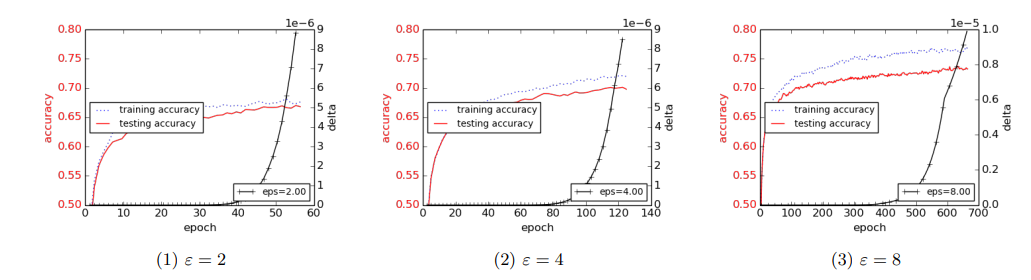
\includegraphics[width=\textwidth]{dp-sgd_results.PNG}
    \caption{DP-SGD Results on CIFAR-10 \cite{Abadi_2016_DeepLearningDifferentialPrivacy}}
    \label{fig:image_label}
\end{figure}

\subsection{Related Work: DP-RMSProp and DP-Adam}\label{subsec:related-work-RMSProp}
For comparison of DP-RMSProp and DP-Adam, we turn to the results from Zhou et al. (2020) \cite{zhou_2020_private_adaptive_algorithms} and Tang et al. (2023) \cite{tang2023dpadambcdpadamactuallydpsgd}.
These 2 papers illustrate some situations where DP-Adam and DP-RMSProp greatly outperform DP-SGD. They also show that these algorithms perform
very similarly on other tasks, specifically on CIFAR-10 in many cases.

\begin{figure}[ht]
    \centering
    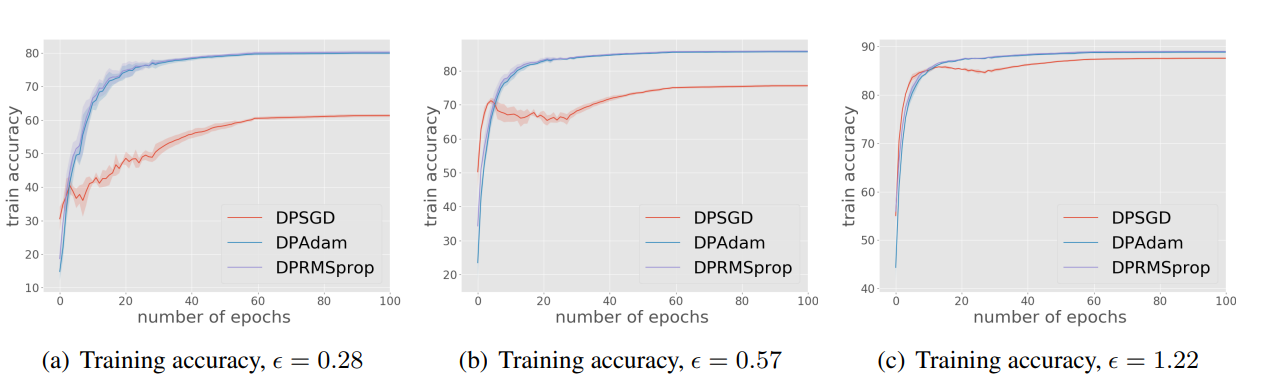
\includegraphics[width=\textwidth]{zhou.PNG}
    \caption{DP-Adam Results on CIFAR-10 \cite{tang2023dpadambcdpadamactuallydpsgd}}
    \label{fig:image_label}
\end{figure}

\begin{figure}[ht]
    \centering
    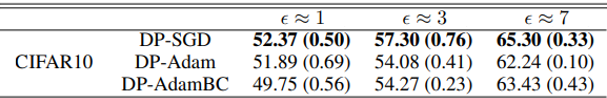
\includegraphics[width=\textwidth]{dp-adam-rms-results.PNG}
    \caption{DP-Adam Results on CIFAR-10 \cite{tang2023dpadambcdpadamactuallydpsgd}}
    \label{fig:image_label}
\end{figure}
    \section{Related Work}\label{sec:related-work}

    \section{Preliminary Results}\label{sec:prelim-results}
    % \subsection{Optimizer Details (with Hyperparameter values)}\label{subsec:optimizer-details}

\subsection{DP Details (Budget Accounting, Noise Scale, No. Iterations)}\label{subsec:dp-details}
\begin{itemize}
    \item \textbf{Budget Accounting:} 
    \item \textbf{Noise Scale:}
    \item \textbf{Number of Iterations:}
\end{itemize}

 
    \section{Discussion of Results}\label{sec:results-discussion}
    % \subsection{Train/Test Loss/Accuracy with varied Epochs}\label{subsec:train-testloss-accuracy}
\begin{itemize}
    \item \textbf{Accuracy/Training Loss:} Accuracy and training loss on CIFAR-10~\cite{cifar10_dataset}.
    \item \textbf{Privacy Cost:} We will measure $(\epsilon, \delta)$ using RDP~\cite{Mironov_2017_RenyiDP} to ensure privacy compliance.
    \item \textbf{Training Time:} Time complexity and memory usage will be tracked.
\end{itemize}

\subsection{Ablation Study}\label{subsec:ablation-study}

\subsection{Graphs showing effects of Hyperparameters}\label{subsec:graphs-hyperparamters}

\subsection{Tables summarizing results (with standard deviation)}\label{subsec:summary-table-results}


    \section{Learned and Plans}\label{sec:learned-and-plans}
    \subsection{Learned}\label{subsec:optimizer-details}

    \bibliographystyle{plain}
    \bibliography{references}

    \section*{GitHub Contributions}
    The code and related materials for this project are available at our GitHub repository:
    \url{https://github.com/CS8960-Privacy-Preserving-Data-Analysis/final-project}.
    Contributions, issues, and discussions are welcome.

    \break
    \section*{Appendix A: Full Model Results}
    \begin{table}[!ht]
        \caption{Experimental Results\\All experiments were conducted with a constant privacy budget $\delta = 10^{-5}$, momentum $\beta = 0.9$, weight decay $\lambda = 10^{-4}$ and a maximum gradient norm of $C = 1.0$.}
        \centering  
        \resizebox{\textwidth}{!}{  
            \begin{tabular}{|c|c|c|c|c|c|c|c|c|}
                \hline
                \textbf{Experiment ID} & \textbf{Optimizer} & \textbf{Epochs} & \textbf{Accuracy} & \textbf{Training Time (s)} & \textbf{Privacy Cost} & \textbf{Learning Rate} & \textbf{Batch Size} & \textbf{Noise Multiplier} \\ [0.5ex]
                \hline\hline
                1  & SGD      & 100 & 87\%    & -       & -      & 0.1  & 128  & -  \\
                2  & SGD      & 200 & 94\%    & -       & -      & 0.1  & -    & -  \\
                3  & DP-SGD   & 30  & 41\%    & 481.49  & 3      & 0.1  & 128  & 1.1 \\
                4  & DP-SGD   & 30  & 40\%    & 598.68  & 3      & 0.2  & 128  & 1.1 \\
                5  & DP-SGD   & 30  & 39\%    & 527.37  & 3      & 0.3  & 128  & 1.1 \\
                6  & DP-SGD   & 30  & 37\%    & 584.55  & 3      & 0.4  & 128  & 1.1 \\
                7  & DP-SGD   & 30  & 38\%    & 597.60  & 3      & 0.5  & 128  & 1.1 \\
                8  & DP-SGD   & 30  & 35\%    & 995.68  & 3      & 0.1  & 64   & 1.1 \\
                9  & DP-SGD   & 30  & 44\%    & 473.86  & 3      & 0.1  & 256  & 1.1 \\
                10 & DP-SGD   & 30  & 44\%    & 597.29  & 2.99   & 0.1  & 512  & 1.1 \\
                11 & DP-SGD   & 30  & 42\%    & 677.04  & 3      & 0.1  & 1024 & 1.1 \\
                12 & DP-SGD   & 30  & 43\%    & 519.55  & 8.01   & 0.1  & 128  & 1.1 \\
                13 & DP-SGD   & 30  & 44\%    & 627.49  & 10.01  & 0.1  & 128  & 1.1 \\
                14 & DP-SGD   & 30  & 48\%    & 553.12  & 50.04  & 0.1  & 128  & 0.1 \\
                15 & DP-SGD   & 30  & 50\%    & 375.37  & 50.04  & 0.1  & 256  & 0.1 \\
                16 & DP-Adam  & 30  & 42\%    & 852.44  & 3      & 0.1  & 128  & 1.1 \\
                17 & DP-Adam  & 30  & 35.55\% & 1426.00 & 3      & 0.1  & 64   & 1.1 \\
                18 & DP-Adam  & 30  & 45\%    & 686.00  & 3      & 0.1  & 256  & 1.1 \\
                19 & DP-Adam  & 30  & 45\%    & 688.00  & 3      & 0.1  & 512  & 1.1 \\
                20 & DP-Adam  & 30  & 42.30\% & 740.00  & 3      & 0.1  & 1024 & 1.1 \\
                21 & DP-Adam  & 30  & 40.13\% & 713.50  & 3      & 0.2  & 128  & 1.1 \\
                22 & DP-Adam  & 30  & 39.34\% & 725.00  & 3      & 0.3  & 128  & 1.1 \\
                23 & DP-Adam  & 30  & 36.80\% & 717.70  & 3      & 0.4  & 128  & 1.1 \\
                24 & DP-Adam  & 30  & 38.28\% & 733.40  & 3      & 0.5  & 128  & 1.1 \\
                25 & DP-Adam  & 30  & 30\%    & 642.00  & 3      & 0.2  & 256  & 1.1 \\
                26 & DP-Adam  & 30  & 38\%    & 690.00  & 10     & 0.1  & 256  & 1.1 \\
                27 & DP-Adam  & 30  & 39\%    & 743.00  & 50     & 0.1  & 256  & 1.1 \\
                28 & DP-Adam  & 100 & 36\%    & 2247.00 & 3      & 0.1  & 256  & 1.1 \\
                32 & RMSProp  & 30  & 42\%    & 459.73  & 3      & 0.01 & 128  & 1.1 \\
                33 & RMSProp  & 30  & 43\%    & 673.73  & 3      & 0.01 & 256  & 1.1 \\
                34 & RMSProp  & 30  & 48\%    & 684.61  & 7.99   & 0.01 & 256  & 1.1 \\
                35 & RMSProp  & 30  & 45\%    & 684.67  & 10     & 0.01 & 256  & 1.1 \\
                36 & RMSProp  & 30  & 44\%    & 667.19  & 3      & 0.01 & 256  & 0.1 \\
                37 & RMSProp  & 30  & 39\%    & 669.75  & 3      & 0.1  & 256  & 1.1 \\
                38 & RMSProp  & 30  & 44\%    & 664.00  & 3      & 0.005 & 256 & 1.1 \\
                39 & RMSProp  & 30  & 46\%    & 674.38  & 7.99   & 0.005 & 256 & 0.1 \\
                40 & RMSProp  & 30  & 45\%    & 672.98  & 8      & 0.01  & 256 & 0.1 \\
                41 & RMSProp  & 30  & 47\%    & 772.55  & 8.01   & 0.01  & 128 & 1.1 \\
                42 & RMSProp  & 30  & 39\%    & 772.55  & 3      & 0.01  & 128 & 0.1 \\
                43 & RMSProp  & 30  & 42\%    & 759.14  & 3      & 0.005 & 128 & 1.1 \\
                44 & RMSProp  & 30  & 45\%    & 775.69  & 8      & 0.005 & 128 & 1.1 \\
                45 & RMSProp  & 30  & 41\%    & 1283.99 & 8      & 0.001 & 64  & 1.1 \\
                46 & RMSProp  & 30  & 44.65\% & 544.07  & 3      & 0.01  & 512 & 1.1 \\
                47 & RMSProp  & 30  & 43.82\% & 756.23  & 3      & 0.01  & 1024 & 1.1 \\
                \hline
            \end{tabular}
        }
        \label{tab:exp_results}
    \end{table}


\end{document}

